\chapter{Le développement végétatif des plantes~: méristèmes et croissance}\label{ch:b2:plant-meristems}

Un chêne qui était une plantule lorsqu'on construisait la cathédrale
ajoute encore un cerne de \omterm{def:b2:plant-meristems:wood}{bois} chaque année, ouvre encore de nouvelles
feuilles à chaque printemps, pousse encore de nouvelles extrémités de
racines à travers le sol. Aucun animal ne fait cela~; un cheval cesse de
grandir à quatre ans. La différence tient à ce qu'une plante conserve, à
l'extrémité de chaque pousse et de chaque racine et dans un mince
cylindre à l'intérieur de chaque tronc, de petites populations de
cellules embryonnaires --- les \emph{\omterm{def:b2:plant-meristems:meristem}{méristèmes}} --- qui ne cessent
jamais de se diviser et qui construisent le corps de la plante vers
l'extérieur et vers le haut aussi longtemps qu'elle vit. Ce chapitre
examine comment les deux \omterm{def:b2:plant-meristems:meristem}{méristèmes} apicaux sont organisés et contrôlés,
comment croît une cellule végétale, comment les hormones décident de la
forme d'une pousse, et comment un tronc s'épaissit.

\section{Les méristèmes}

\begin{definition}[Les méristèmes et les deux types de croissance]\label{def:b2:plant-meristems:meristem}
\index{meristeme@méristème}\index{meristeme apical caulinaire@méristème apical caulinaire}\index{meristeme apical racinaire@méristème apical racinaire}\index{cambium}
Un \emph{méristème} est une population de petites cellules
indifférenciées en division, qui persiste pendant toute la vie de la
plante et dont dérivent tous ses tissus. Le \emph{méristème apical
caulinaire} (MAC), à l'extrémité de chaque pousse, produit les
feuilles, la tige et, à la bonne saison, les \omterm{def:b2:angiosperm-reproduction:flower}{fleurs}~; le \emph{méristème
apical racinaire} (MAR), derrière chaque extrémité de racine, produit
la racine~; ensemble, ils assurent la \emph{croissance primaire},
l'allongement de la plante. Les \emph{méristèmes latéraux} --- le
\emph{cambium} et le \emph{phellogène}, minces cylindres situés à
l'intérieur des tiges et des racines --- assurent la \emph{croissance
secondaire}, l'épaississement qui produit le \omterm{def:b2:plant-meristems:wood}{bois} et l'\omterm{def:b2:plant-meristems:wood}{écorce}. La
croissance des plantes est donc \emph{indéfinie}~: les méristèmes
peuvent fonctionner indéfiniment, et la plante est un organisme
modulaire, qui répète l'unité feuille--nœud--entre-nœud--bourgeon tant
que les conditions le permettent. Chaque bourgeon axillaire est un MAC
dormant~: une plante porte ainsi des milliers de points de croissance
de réserve.
\end{definition}

\begin{proposition}[L'apex caulinaire]\label{prop:b2:plant-meristems:sam}
\index{phyllotaxie}\index{primordium foliaire}\index{plastochrone}
Le MAC est un dôme d'un dixième de millimètre de diamètre, formé de
quelques centaines de cellules. Ses une ou deux couches externes (la
\emph{tunica}) ne se divisent que dans le plan de la surface et donnent
l'épiderme~; la masse sous-jacente (le \emph{corpus}) se divise dans
tous les plans. Au sommet, une \emph{zone centrale} de \omterm{def:b2:cell-differentiation:differentiation}{cellules souches}
à division lente alimente une \emph{zone périphérique} de cellules à
division plus rapide, où des \emph{\omterm{prop:b2:plant-meristems:sam}{primordiums foliaires}} apparaissent
sous forme de renflements à intervalles de temps réguliers (le
\emph{plastochrone}, de quelques heures à quelques jours) et selon des
angles réguliers autour du dôme (la \emph{phyllotaxie}~: opposée,
verticillée, ou spiralée selon l'angle d'or de \qty{137.5}{\degree}, qui
place chaque nouvelle feuille dans le plus grand espace laissé par les
autres). En dessous, une \emph{zone médullaire} produit la moelle et
allonge la tige. Un primordium se forme là où l'hormone auxine
s'accumule dans la couche superficielle et, en grandissant, il draine
l'auxine de son voisinage~: c'est pourquoi le primordium suivant apparaît
aussi loin de lui que possible. Le motif s'auto-organise.
\end{proposition}

\begin{omfigure}
\begin{tikzpicture}[every node/.style={font=\scriptsize}]
  % dome
  \draw[thick, fill=omExo!12] (-2.2,0) .. controls (-2.2,1.6) and (-0.8,2.6) .. (0,2.6) .. controls (0.8,2.6) and (2.2,1.6) .. (2.2,0) -- (2.2,-1.4) -- (-2.2,-1.4) -- cycle;
  % tunica layers
  \draw[thick, omDef] (-2.2,0) .. controls (-2.2,1.5) and (-0.8,2.45) .. (0,2.45) .. controls (0.8,2.45) and (2.2,1.5) .. (2.2,0);
  \draw[thick, omDef] (-2.05,0) .. controls (-2.05,1.35) and (-0.75,2.3) .. (0,2.3) .. controls (0.75,2.3) and (2.05,1.35) .. (2.05,0);
  % zones
  \draw[thick, dashed, omThm, fill=omThm!15] (0,1.75) ellipse (0.6 and 0.55);
  \draw[thick, dashed, omProp] (0,0.9) ellipse (1.6 and 1.35);
  \draw[thick, dashed, omExo!70!black] (-0.9,-0.9) rectangle (0.9,-0.1);
  % primordia
  \draw[thick, fill=omExo!40] (-2.2,0.4) .. controls (-2.5,1.4) and (-1.6,1.9) .. (-1.55,1.3) .. controls (-1.5,0.9) and (-1.9,0.6) .. (-2.2,0.4);
  \draw[thick, fill=omExo!40] (2.2,0.2) .. controls (2.7,1.0) and (2.1,1.5) .. (1.75,1.1) .. controls (1.6,0.8) and (1.9,0.5) .. (2.2,0.2);
  % labels
  \draw (0.4,2.1) -- (3.2,2.6) node[right, align=left] {zone centrale~:\\cellules souches à division lente};
  \draw (1.3,0.5) -- (3.2,1.4) node[right, align=left] {zone périphérique~:\\division rapide, primordiums foliaires};
  \draw (0.6,-0.5) -- (3.2,0.0) node[right, align=left] {zone médullaire~: moelle,\\allongement de la tige};
  \draw (-1.7,1.5) -- (-3.0,2.4) node[left, align=right] {primordium\\foliaire};
  \draw (-1.2,2.05) -- (-3.0,1.2) node[left, align=right] {tunica~: divisions\\superficielles seulement};
  \draw (2.2,0.7) -- (3.2,-1.0) node[right, align=left] {primordium suivant,\\à \qty{137.5}{\degree}};
\end{tikzpicture}

{\small Le \omterm{def:b2:plant-meristems:meristem}{méristème apical caulinaire} en coupe~: une tunica d'une ou
deux couches superficielles au-dessus d'un corpus, une zone centrale de
\omterm{def:b2:cell-differentiation:differentiation}{cellules souches} au sommet, une zone périphérique où bombent les
\omterm{prop:b2:plant-meristems:sam}{primordiums foliaires}, et une zone médullaire en dessous.}
\end{omfigure}

\begin{omfigure}
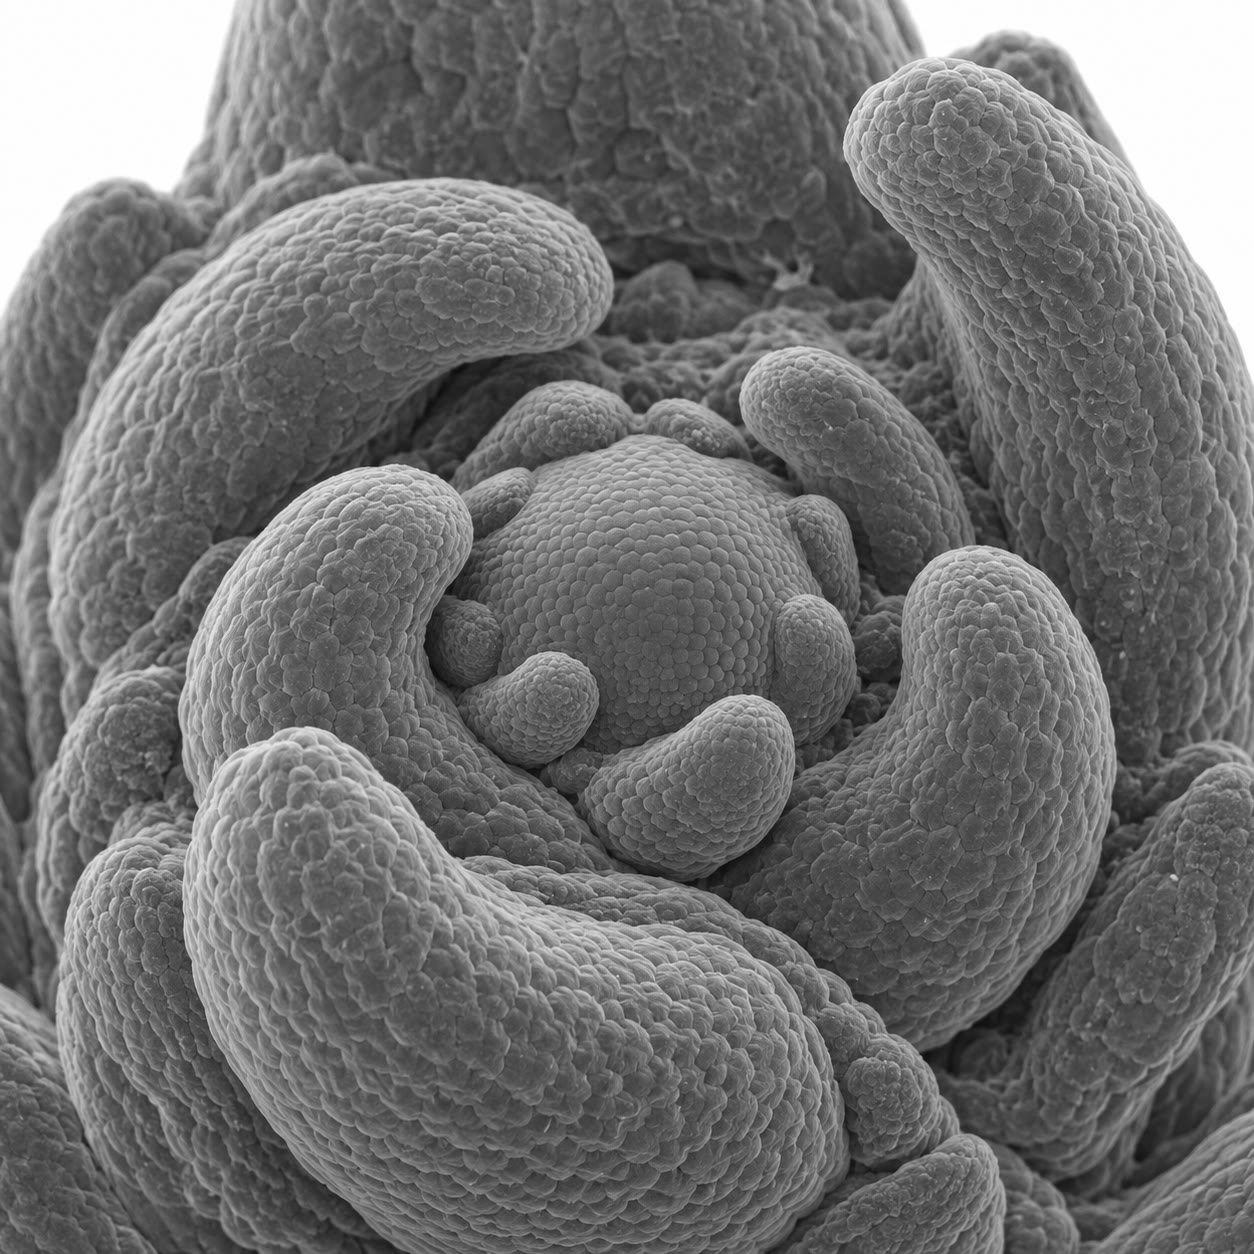
\includegraphics[width=0.44\linewidth]{images/book4/ai/b4-13-shoot-apex-sem.jpg}

{\small Un apex caulinaire au microscope électronique à balayage~: le
dôme lisse du \omterm{def:b2:plant-meristems:meristem}{méristème} et la spirale de \omterm{prop:b2:plant-meristems:sam}{primordiums foliaires} qui
l'entoure, chaque nouveau primordium placé dans le plus grand espace
libre.}
\end{omfigure}

\begin{proposition}[Maintenir les cellules souches~: une boucle de rétroaction]\label{prop:b2:plant-meristems:wus}
\index{WUSCHEL}\index{CLAVATA}\index{retroaction negative!meristeme@rétroaction négative!méristème}
La taille du stock de \omterm{def:b2:cell-differentiation:differentiation}{cellules souches} est maintenue constante par une
boucle entre deux gènes. Les cellules situées juste sous la zone
centrale expriment le \omterm{prop:b2:cell-differentiation:transcriptional}{facteur de transcription} \emph{WUSCHEL} (WUS), dont
le produit migre vers les cellules sus-jacentes et les maintient à
l'état de \omterm{def:b2:cell-differentiation:differentiation}{cellules souches}~; les \omterm{def:b2:cell-differentiation:differentiation}{cellules souches} sécrètent en retour un
petit peptide, \emph{CLAVATA3} (CLV3), qui diffuse vers le bas, se fixe
sur un récepteur kinase (CLV1) des cellules exprimant WUS et réprime
WUS. Plus de \omterm{def:b2:cell-differentiation:differentiation}{cellules souches} signifie plus de CLV3, moins de WUS, moins
de \omterm{def:b2:cell-differentiation:differentiation}{cellules souches}~; moins de \omterm{def:b2:cell-differentiation:differentiation}{cellules souches} signifie moins de CLV3,
plus de WUS, plus de \omterm{def:b2:cell-differentiation:differentiation}{cellules souches}. Le stock est ainsi une grandeur
régulée, comme les gonadotrophines du
\cref{ch:b2:reproductive-hormones}, et la même logique --- un signal émis
par la population régulée qui réprime le facteur qui la produit ---
maintient aussi le \omterm{def:b2:plant-meristems:meristem}{méristème} racinaire.
\end{proposition}
\begin{proof}[Faits expérimentaux]
Les mutants \emph{clavata} d'Arabidopsis (Clark, Meyerowitz, années
1990) ont des \omterm{def:b2:plant-meristems:meristem}{méristèmes} qui gonflent jusqu'à plusieurs fois la taille
normale, avec des feuilles surnuméraires, des pièces florales
surnuméraires et des tiges fasciées (aplaties, en ruban)~: le frein a
disparu. Les mutants \emph{wuschel} forment un \omterm{def:b2:plant-meristems:meristem}{méristème} qui s'arrête
après quelques feuilles, puis en forment de nouveaux, qui s'arrêtent à
leur tour~: l'accélérateur a disparu. Chez le double mutant, le
\omterm{def:b2:meiosis-heredity:vocabulary}{phénotype} \emph{wuschel} l'emporte, ce qui place WUS en aval de CLV~; et
le peptide CLV3 appliqué sur un apex sauvage réprime WUS en quelques
heures.
\end{proof}

\begin{proposition}[L'apex racinaire]\label{prop:b2:plant-meristems:ram}
\index{coiffe}\index{centre quiescent}\index{zone d'elongation@zone d'élongation}\index{poil absorbant}
Une racine croît à partir d'un \omterm{def:b2:plant-meristems:meristem}{méristème} abrité derrière une
\emph{coiffe}, dont les cellules desquament à mesure que l'extrémité
progresse dans le sol, et qui sécrète un mucilage lubrifiant et perçoit
la gravité (grains d'amidon qui sédimentent dans ses cellules). Au
centre du \omterm{def:b2:plant-meristems:meristem}{méristème}, un \emph{\omterm{prop:b2:plant-meristems:ram}{centre quiescent}} de quelques centaines
de cellules ne se divise que rarement~; il maintient à l'état de
\omterm{def:b2:cell-differentiation:differentiation}{cellules souches} les initiales qui l'entourent --- celles de la coiffe,
de l'épiderme, du parenchyme cortical et du cylindre central --- comme
WUS maintient celles de la pousse. Derrière le \omterm{def:b2:plant-meristems:meristem}{méristème} vient la
\emph{\omterm{prop:b2:plant-meristems:ram}{zone d'élongation}}, quelques millimètres dans lesquels les
cellules s'allongent de dix à vingt fois, poussant l'extrémité en
avant~; puis la \emph{zone de \omterm{def:b2:cell-differentiation:differentiation}{différenciation}}, où l'épiderme forme des
\emph{\omterm{prop:b2:plant-meristems:ram}{poils absorbants}} et où le xylème et le phloème mûrissent. Les
racines latérales ne naissent pas à l'extrémité mais du péricycle, au
cœur de la racine mûre, en face des pôles du xylème, et traversent le
parenchyme cortical pour sortir. L'auxine, produite dans la pousse et
transportée vers le bas, s'accumule à l'extrémité et organise
l'ensemble~; le \omterm{prop:b2:plant-meristems:ram}{centre quiescent} se trouve à son maximum.
\end{proposition}

\begin{omfigure}
\begin{tikzpicture}[every node/.style={font=\scriptsize}]
  % root outline
  \draw[thick, fill=omExo!10] (-1.0,4.5) -- (-1.0,0.6) .. controls (-1.0,-0.4) and (1.0,-0.4) .. (1.0,0.6) -- (1.0,4.5);
  % root cap
  \draw[thick, fill=omExo!45] (-0.9,0.8) .. controls (-1.1,-0.1) and (1.1,-0.1) .. (0.9,0.8) .. controls (0.5,0.4) and (-0.5,0.4) .. (-0.9,0.8);
  % meristem
  \fill[omThm!25] (-0.85,0.8) rectangle (0.85,1.7);
  \fill[omThm!70] (0,0.95) ellipse (0.25 and 0.12);
  % elongation zone
  \fill[omProp!20] (-0.85,1.7) rectangle (0.85,3.0);
  % differentiation zone with root hairs and vascular strand
  \fill[omDef!15] (-0.85,3.0) rectangle (0.85,4.5);
  \fill[omDef!50] (-0.15,3.0) rectangle (0.15,4.5);
  \foreach \y in {3.2,3.5,3.8,4.1,4.4} { \draw[omDef!80!black] (1.0,\y) -- (1.7,\y+0.1); \draw[omDef!80!black] (-1.0,\y) -- (-1.7,\y+0.1); }
  % lateral root primordium
  \draw[thick, fill=omThm!30] (0.15,4.0) .. controls (0.5,3.9) and (0.8,4.1) .. (0.9,4.3) .. controls (0.7,4.35) and (0.4,4.3) .. (0.15,4.3);
  % labels
  \draw (0.5,0.4) -- (2.2,0.2) node[right] {coiffe};
  \draw (0.25,0.95) -- (2.2,0.9) node[right] {centre quiescent};
  \draw (0.85,1.4) -- (2.2,1.5) node[right] {méristème (division)};
  \draw (0.85,2.4) -- (2.2,2.3) node[right, align=left] {zone d'élongation~:\\allongement des cellules $10\times$};
  \draw (1.5,3.6) -- (2.2,3.4) node[right] {poils absorbants};
  \draw (0.0,4.2) -- (2.2,4.2) node[right] {cylindre central};
  \draw (0.7,4.3) -- (2.2,4.9) node[right, align=left] {primordium de racine latérale\\(issu du péricycle)};
  \draw[->, thick] (-2.4,4.5) -- (-2.4,0.6); \node[left, rotate=90, anchor=south] at (-2.5,2.5) {l'auxine descend vers l'extrémité};
\end{tikzpicture}

{\small L'extrémité de la racine~: coiffe, \omterm{def:b2:plant-meristems:meristem}{méristème} et son \omterm{prop:b2:plant-meristems:ram}{centre
quiescent}, \omterm{prop:b2:plant-meristems:ram}{zone d'élongation}, et zone de \omterm{def:b2:cell-differentiation:differentiation}{différenciation} avec les \omterm{prop:b2:plant-meristems:ram}{poils
absorbants} et les vaisseaux mûrs. Les racines latérales naissent en
profondeur, à partir du péricycle.}
\end{omfigure}

\begin{omfigure}
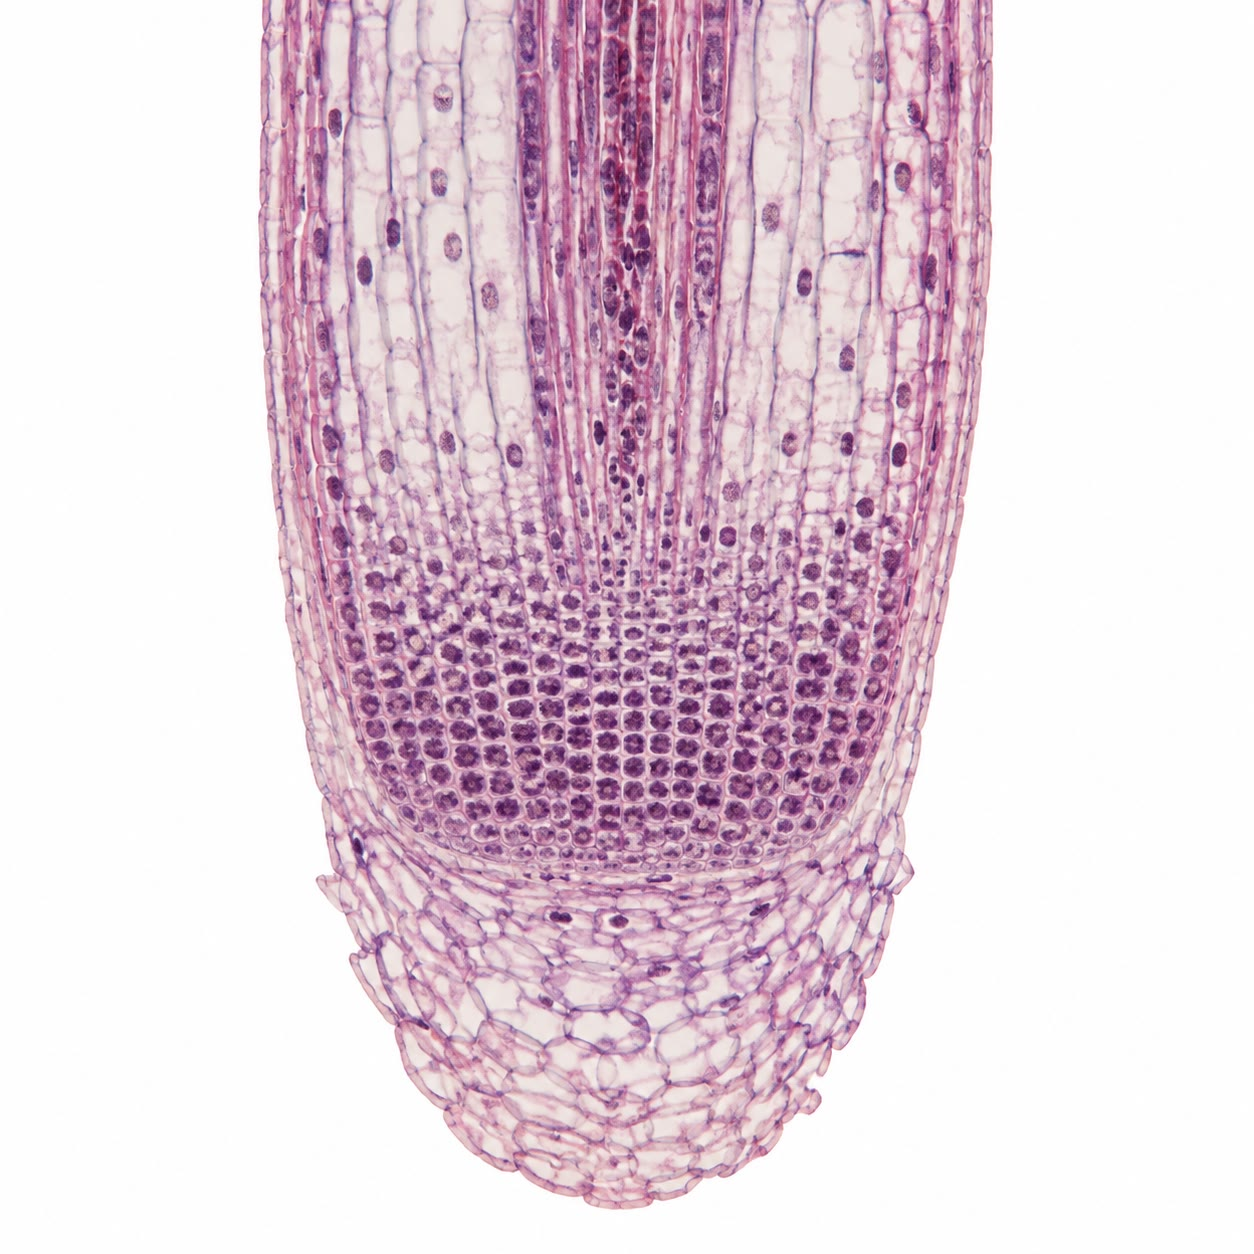
\includegraphics[width=0.42\linewidth]{images/book4/ai/b4-13-root-tip.jpg}

{\small Une extrémité de racine en coupe longitudinale~: les cellules
lâches de la coiffe, le \omterm{def:b2:plant-meristems:meristem}{méristème} dense aux noyaux sombres, et les
cellules en allongement au-dessus.}
\end{omfigure}

\section{Comment croît une cellule végétale}

\begin{theorem}[L'équation de Lockhart]\label{thm:b2:plant-meristems:lockhart}
\index{turgescence}\index{paroi!extensibilite@extensibilité}\index{equation de Lockhart@équation de Lockhart}
Une cellule végétale croît en étirant sa paroi sous la pression de son
propre contenu. La paroi ne cède de façon irréversible qu'au-dessus
d'une turgescence seuil $Y$, et alors à une vitesse proportionnelle à
l'excédent~: la vitesse relative de croissance d'une cellule de longueur
$L$ est
\[
\frac{1}{L}\frac{\mathrm{d}L}{\mathrm{d}t} = \phi\,(P - Y) \quad (P > Y),
\]
où $P$ est la pression de turgescence et $\phi$ l'\emph{extensibilité}
de la paroi. La croissance est donc contrôlée de deux côtés~: par l'eau,
qui fixe $P$ (une cellule qui flétrit cesse de croître), et par la
paroi, qui fixe $\phi$ et $Y$ --- et c'est sur la paroi qu'agissent les
hormones. L'auxine fait pomper des protons dans la paroi par les
cellules~; l'acidité active les \emph{expansines}, des protéines qui
relâchent les liaisons entre les fibrilles de cellulose et la matrice,
ce qui élève $\phi$ et abaisse $Y$ en quelques minutes (\emph{croissance
acide}). Avec $\phi =
\qty{0.1}{h^{-1}.MPa^{-1}}$, $Y = \qty{0.3}{MPa}$ et $P =
\qty{0.6}{MPa}$, une cellule s'allonge de \qty{3}{\%} par heure et
double en une journée~; dans la \omterm{prop:b2:plant-meristems:ram}{zone d'élongation} d'une racine, où les
vitesses sont plusieurs fois plus élevées, une cellule s'allonge de dix
fois en quelques heures.
\end{theorem}
\begin{proof}
La paroi est un matériau viscoplastique~: en dessous de la contrainte
seuil, elle se déforme élastiquement et revient à sa forme~; au-dessus,
elle flue à une vitesse proportionnelle à l'excès de contrainte. La
contrainte dans la paroi est proportionnelle à la pression de
turgescence (pour un cylindre de rayon $r$ et de paroi d'épaisseur $w$,
la contrainte circonférentielle vaut $Pr/w$)~: la vitesse de
déformation plastique est donc proportionnelle à $P - Y$, avec une
constante $\phi$ qui intègre la géométrie et les propriétés du matériau
pariétal. La vitesse de déformation est par définition
$(1/L)\,\mathrm{d}L/\mathrm{d}t$. Numériquement,
$0.1\times(0.6 - 0.3) = \qty{0.03}{h^{-1}}$, et $L$ double lorsque
$0.03\,t = \ln 2$, $t = \qty{23}{h}$.
\end{proof}

\begin{omfigure}
\begin{tikzpicture}
\begin{axis}[
  width=0.7\linewidth, height=5.4cm,
  axis x line=bottom, axis y line=left,
  xmin=0, xmax=1.0, ymin=0, ymax=0.09,
  xlabel={pression de turgescence $P$ (\unit{MPa})}, ylabel={vitesse relative de croissance (\unit{h^{-1}})},
  xlabel style={font=\small, at={(axis description cs:0.5,-0.13)}, anchor=north},
  ylabel style={font=\small},
  tick label style={font=\small}, xtick={0,0.3,0.6,0.9}, ytick={0,0.03,0.06,0.09},
  yticklabels={0,0.03,0.06,0.09}, scaled y ticks=false,
  legend style={font=\scriptsize, at={(0.03,0.97)}, anchor=north west, draw=none},
  clip=false,
]
\addplot[very thick, omDef, domain=0:0.3, samples=2, forget plot] {0};
\addplot[very thick, omDef, domain=0.3:1.0, samples=2] {0.1*(x-0.3)};
\addlegendentry{$\phi = 0.1$, $Y = 0.3$}
\addplot[very thick, omThm, domain=0:0.2, samples=2, forget plot] {0};
\addplot[very thick, omThm, domain=0.2:0.65, samples=2] {0.2*(x-0.2)};
\addlegendentry{avec auxine~: $\phi = 0.2$, $Y = 0.2$}
\draw[dashed, gray] (axis cs:0.6,0) -- (axis cs:0.6,0.03); \node[font=\scriptsize, anchor=west] at (axis cs:0.61,0.015) {$P$ typique};
\end{axis}
\end{tikzpicture}

{\small La loi de Lockhart~: pas de croissance en dessous de la
turgescence seuil, puis une vitesse proportionnelle à l'excédent.
L'auxine, en relâchant la paroi, abaisse le seuil et accentue la pente~:
à turgescence égale, la cellule croît plusieurs fois plus vite.}
\end{omfigure}

\begin{example}[D'où vient l'eau]\label{ex:b2:plant-meristems:water}
À mesure que la paroi cède, la turgescence chuterait et la croissance
s'arrêterait si de l'eau n'entrait pas au même rythme~: la cellule en
croissance est une fuite qui se remplit d'elle-même. L'eau vient du
xylème, le long d'un faible gradient de potentiel hydrique, et sa
vitesse d'entrée est fixée par la conductance hydraulique de la
membrane~; la croissance est maximale la nuit, quand la transpiration
est faible et la turgescence élevée, et une feuille de maïs peut
s'allonger de \qty{10}{cm} entre le crépuscule et l'aube. En cas de
sécheresse, les cellules fabriquent des solutés (\emph{ajustement
osmotique}) pour maintenir $P$ au-dessus de $Y$, et lorsque cela
échoue, la feuille cesse de croître des jours avant de flétrir.
\end{example}

\section{Les hormones et la forme de la pousse}

\begin{proposition}[L'auxine et la dominance apicale]\label{prop:b2:plant-meristems:apical}
\index{auxine}\index{dominance apicale}\index{transport polarise de l'auxine@transport polarisé de l'auxine}\index{cytokinine}
L'\emph{auxine} (acide indole-3-acétique) est produite dans l'apex
caulinaire et les jeunes feuilles et transportée vers le bas de la
tige, de cellule en cellule, à environ \qty{1}{cm/h}, par des protéines
de transport (PIN) placées à l'extrémité inférieure de chaque cellule
--- un \emph{transport polarisé} qui donne à la plante un axe
haut-bas. Le flux d'auxine qui descend de l'apex maintient en \omterm{def:b2:angiosperm-reproduction:seed}{dormance}
les bourgeons axillaires situés au-dessous (\emph{\omterm{prop:b2:plant-meristems:apical}{dominance apicale}}),
en partie en les empêchant d'exporter leur propre auxine vers la tige,
en partie en induisant des strigolactones et en réprimant les
cytokinines. Coupez l'apex, et les bourgeons les plus proches de la
coupe se développent en quelques jours, donnant une plante buissonnante
--- ce qu'exploitent la taille et le pincement. Les \emph{cytokinines},
produites dans les extrémités des racines et transportées vers le haut
dans le xylème, favorisent le débourrement et la division cellulaire~;
les \emph{gibbérellines} allongent les entre-nœuds (les pois nains et
les blés semi-nains de la révolution verte sont déficients dans leur
synthèse ou leur perception)~; l'acide abscissique et l'éthylène freinent
la croissance en cas de stress. La forme de la pousse --- haute ou
buissonnante, dressée ou étalée --- résulte d'une négociation entre ces
signaux, et l'équilibre entre racines et pousses est fixé par l'auxine
qui descend face aux cytokinines qui montent.
\end{proposition}
\begin{proof}[Faits expérimentaux]
Thimann et Skoog (1934) coupèrent l'apex de plants de haricot~: les
bourgeons latéraux se développèrent. Un bloc de gélose contenant de
l'auxine, posé sur le moignon coupé, les maintint en \omterm{def:b2:angiosperm-reproduction:seed}{dormance} comme
l'avait fait l'apex~; de la gélose seule, non. Went (1928) avait déjà
mesuré l'auxine par la courbure qu'elle provoquait chez des coléoptiles
d'avoine décapités lorsqu'on la plaçait d'un côté du moignon --- le
premier dosage biologique d'une hormone végétale, et l'origine de son
nom, du grec «~croître~». La polarité du transport fut montrée en
plaçant de la gélose à auxine à une extrémité d'un segment de tige et en
ne la retrouvant dans un bloc récepteur à l'autre extrémité que si le
segment était orienté apex vers le haut, quelle que soit l'orientation
du segment dans le champ de pesanteur.
\end{proof}

\begin{omfigure}
\begin{tikzpicture}[every node/.style={font=\scriptsize}, >=stealth]
  \foreach \x/\lab/\apex/\aux in {0/{intacte~: apex en place,\\bourgeons dormants}/1/0, 4.2/{décapitée~:\\les bourgeons débourrent}/0/0, 8.4/{décapitée + auxine\\sur la section~: dormants}/0/1} {
    \begin{scope}[xshift=\x cm]
      \draw[very thick, omExo!70!black] (0,0) -- (0,3.4);
      \foreach \y in {0.8,1.6,2.4} { \draw[thick, omExo!70!black] (0,\y) -- (-0.8,\y+0.4); \draw[thick, omExo!70!black] (0,\y+0.4) -- (0.8,\y+0.8); }
      \ifnum\apex=1 \draw[thick, fill=omThm!40] (0,3.5) ellipse (0.25 and 0.3); \draw[->, thick, omThm] (0.35,3.2) -- (0.35,1.0); \node[omThm, right] at (0.4,2.1) {auxine}; \fi
      \ifnum\apex=0 \draw[thick] (-0.3,3.4) -- (0.3,3.4); \fi
      \ifnum\aux=1 \draw[thick, fill=omThm!40] (-0.25,3.4) rectangle (0.25,3.75); \node[omThm, right] at (0.3,3.6) {gélose à auxine}; \draw[->, thick, omThm] (0.35,3.2) -- (0.35,1.0); \fi
      \ifnum\apex=1 \foreach \y in {0.8,1.6,2.4} \fill[gray!60] (-0.12,\y+0.1) circle (0.08); \fi
      \ifnum\aux=1 \foreach \y in {0.8,1.6,2.4} \fill[gray!60] (-0.12,\y+0.1) circle (0.08); \fi
      \ifnum\apex=0 \ifnum\aux=0 \foreach \y in {0.8,1.6,2.4} { \draw[thick, omExo!70!black] (-0.1,\y+0.1) -- (-0.7,\y+0.9); \draw[thick, omExo!70!black] (-0.7,\y+0.9) -- (-1.0,\y+1.1); \draw[thick, omExo!70!black] (-0.7,\y+0.9) -- (-0.75,\y+1.25); } \fi\fi
      \node[below, align=center] at (0,-0.3) {\lab};
    \end{scope}
  }
\end{tikzpicture}

{\small La \omterm{prop:b2:plant-meristems:apical}{dominance apicale}, l'expérience de Thimann et Skoog. L'apex
maintient les bourgeons axillaires en \omterm{def:b2:angiosperm-reproduction:seed}{dormance}~; son ablation les
libère~; de l'auxine posée sur le moignon remplace l'apex.}
\end{omfigure}

\begin{example}[Signal rapide, molécule lente]\label{ex:b2:plant-meristems:transport}
Le transport polarisé déplace l'auxine de \qty{1}{cm} en une heure~; la
diffusion seule mettrait, pour le même centimètre,
$t = x^2/2D = 10^{-4}/(2\times
10^{-9}) = \qty{5e4}{s}$ --- quatorze heures --- et pour les dix
centimètres qui la séparent d'un bourgeon inférieur, soixante jours. Le
système de pompes et de relais des transporteurs PIN est ce qui rend
un signal hormonal utilisable sur toute la longueur d'une plante~; les
mêmes transporteurs, déplacés vers la face ombragée d'une tige, la font
se courber vers la lumière (\cref{ch:b2:plant-plasticity}).
\end{example}

\section{La croissance secondaire~: bois et écorce}

\begin{definition}[Le cambium et le bois]\label{def:b2:plant-meristems:wood}
\index{cambium!libero-ligneux@libéro-ligneux}\index{bois}\index{cerne annuel}\index{ecorce@écorce}\index{periderme@périderme}
Dans une tige ligneuse, les faisceaux de xylème et de phloème primaires
sont réunis, dès la première année, en un cylindre continu de cellules
en division, le \emph{\omterm{def:b2:plant-meristems:meristem}{cambium}}. Ses cellules se divisent
tangentiellement, ajoutant du \emph{xylème secondaire} --- le
\emph{bois} --- vers l'intérieur et du \emph{phloème secondaire} vers
l'extérieur, si bien que le \omterm{def:b2:plant-meristems:meristem}{cambium} se déplace vers l'extérieur à mesure
que le tronc s'épaissit, et ajoutant de temps à autre des divisions
radiales pour élargir l'anneau. Sous les climats saisonniers, le bois
formé au printemps possède de larges vaisseaux à parois minces (le
\emph{bois initial}) et celui de l'été des vaisseaux étroits à parois
épaisses (le \emph{bois final}), si bien que chaque année laisse un
\emph{cerne annuel} visible~; les cernes enregistrent l'âge de l'arbre
et, par leur largeur, le climat de chaque année (dendrochronologie).
Seuls les cernes externes, l'\emph{aubier}, conduisent la sève~; les
cernes internes, le \emph{duramen}, sont morts, obstrués et assombris
par des résines et des tanins, et servent de squelette à l'arbre. À
l'extérieur du phloème, un second \omterm{def:b2:plant-meristems:meristem}{méristème} latéral, le
\emph{phellogène}, produit le \emph{périderme} --- des couches de
cellules de liège, mortes et imperméabilisées par la subérine --- qui
forme avec l'ancien phloème l'\emph{écorce}. Un tronc est ainsi une
mince enveloppe vivante de \omterm{def:b2:plant-meristems:meristem}{cambium}, d'aubier et de phloème autour d'un
cœur mort, sous une peau morte.
\end{definition}

\begin{omfigure}
\begin{tikzpicture}[every node/.style={font=\scriptsize}]
  \fill[omExo!60] (0,0) circle (3.0);
  \fill[omDef!20] (0,0) circle (2.75);
  \fill[omDef!35] (0,0) circle (2.2);
  \foreach \r in {0.4,0.7,1.0,1.3,1.6,1.9,2.2} \draw[omDef!80!black, thin] (0,0) circle (\r);
  \fill[omExo!80!black] (0,0) circle (1.3);
  \foreach \r in {0.4,0.7,1.0} \draw[omExo!40, thin] (0,0) circle (\r);
  \draw[very thick, omThm] (0,0) circle (2.5);
  \draw (2.9,0.6) -- (3.9,1.6) node[right, align=left] {écorce~: liège (périderme)\\et ancien phloème};
  \draw (2.62,0.0) -- (3.9,0.6) node[right] {phloème secondaire, vivant};
  \draw (2.5,-0.4) -- (3.9,-0.4) node[right] {cambium (en rouge)};
  \draw (1.9,-1.1) -- (3.9,-1.4) node[right, align=left] {aubier~: cernes récents,\\conducteurs};
  \draw (0.5,-0.9) -- (3.9,-2.4) node[right, align=left] {duramen~: cernes anciens,\\morts, obstrués};
  \draw (-1.7,1.5) -- (-3.6,2.4) node[left, align=right] {un cerne annuel~:\\bois initial clair,\\bois final sombre};
\end{tikzpicture}

{\small Un tronc en coupe transversale. Le \omterm{def:b2:plant-meristems:meristem}{cambium} (en rouge) ajoute
chaque année du \omterm{def:b2:plant-meristems:wood}{bois} vers l'intérieur et du phloème vers l'extérieur~;
les cernes récents conduisent la sève, les anciens forment le duramen
mort~; le liège et l'ancien phloème forment l'\omterm{def:b2:plant-meristems:wood}{écorce}.}
\end{omfigure}

\begin{theorem}[Pourquoi un vieil arbre ajoute plus de bois]\label{thm:b2:plant-meristems:rings}
Un tronc de rayon $r$ et de hauteur $h$ dont le \omterm{def:b2:plant-meristems:meristem}{cambium} ajoute chaque
année un cerne d'épaisseur $\Delta r$ gagne un volume de \omterm{def:b2:plant-meristems:wood}{bois}
\[
\Delta V \approx 2\pi r\,h\,\Delta r
\]
par an~: pour une largeur de cerne constante, l'accroissement annuel
croît proportionnellement au rayon, et un arbre de \qty{50}{cm} de rayon
ajoute dix fois plus de \omterm{def:b2:plant-meristems:wood}{bois} qu'un arbre de \qty{5}{cm}, bien que ses
cernes ne soient pas plus larges. Un tronc de \qty{25}{cm} de rayon et
de \qty{10}{m} de hauteur qui s'épaissit de \qty{4}{mm} par an gagne
\qty{0.063}{m^3}, soit environ \qty{30}{kg} de \omterm{def:b2:plant-meristems:wood}{bois} sec ---
\qty{15}{kg} de carbone, puisés dans l'air par la couronne en une
saison.
\end{theorem}
\begin{proof}
Le \omterm{def:b2:plant-meristems:wood}{bois} ajouté est une enveloppe cylindrique de circonférence $2\pi r$,
d'épaisseur $\Delta r$ et de hauteur $h$~; son volume vaut
$2\pi r h\Delta r$ au premier ordre en $\Delta r$ (exactement
$\pi h[(r + \Delta r)^2 - r^2]
= \pi h(2r\Delta r + \Delta r^2)$). Avec $r = 0.25$, $h = 10$,
$\Delta r = 0.004$~: $2\pi\times 0.25\times 10\times 0.004 =
\qty{0.063}{m^3}$~; à \qty{500}{kg/m^3} de \omterm{def:b2:plant-meristems:wood}{bois} sec, \qty{31}{kg}, dont
la moitié de carbone.
\end{proof}

\begin{omfigure}
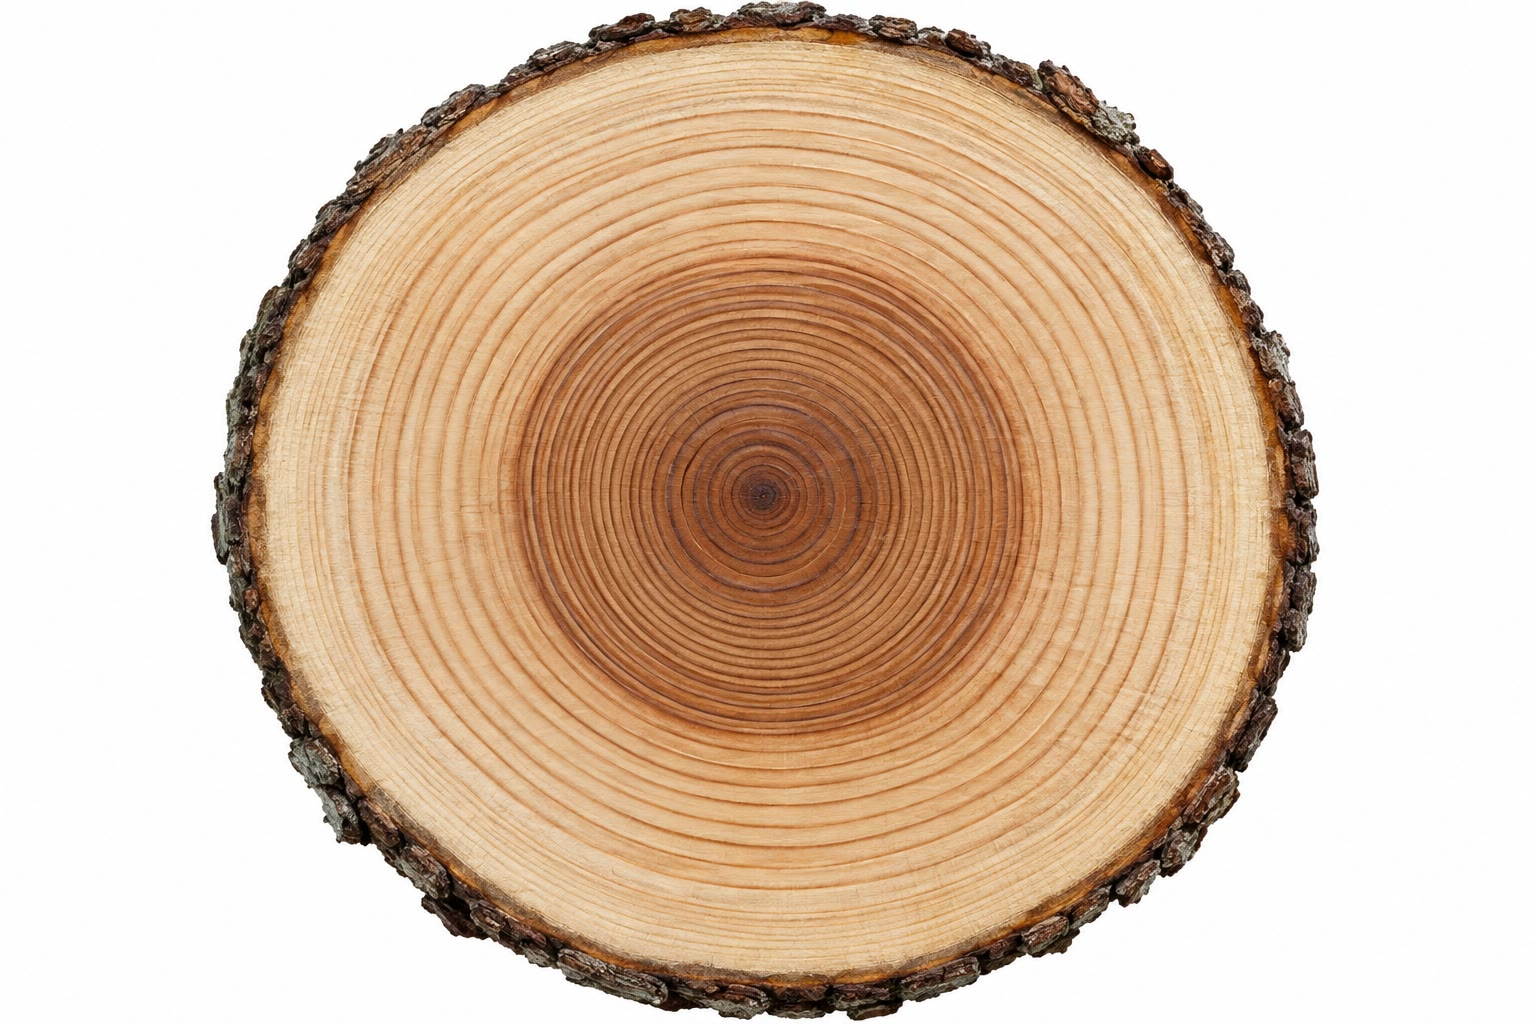
\includegraphics[width=0.5\linewidth]{images/book4/ai/b4-13-wood-rings.jpg}

{\small Un tronc de pin en coupe transversale~: les \omterm{def:b2:plant-meristems:wood}{cernes annuels}, chacun
formé d'une bande claire de \omterm{def:b2:plant-meristems:wood}{bois} initial et d'une bande sombre de \omterm{def:b2:plant-meristems:wood}{bois}
final, le duramen plus sombre, et l'\omterm{def:b2:plant-meristems:wood}{écorce}.}
\end{omfigure}

\section{Exercices}

\begin{exercise}[$\star$]\label{exo:b2:plant-meristems:1}
Définir un \omterm{def:b2:plant-meristems:meristem}{méristème}, et nommer les quatre \omterm{def:b2:plant-meristems:meristem}{méristèmes} d'une plante
ligneuse avec ce que produit chacun.
\end{exercise}

\begin{exercise}[$\star$]\label{exo:b2:plant-meristems:2}
Énumérer les zones d'une extrémité de racine, de la coiffe vers le
haut, avec ce qui arrive à une cellule dans chacune. D'où viennent les
racines latérales~?
\end{exercise}

\begin{exercise}[$\star$]\label{exo:b2:plant-meristems:3}
Décrire l'expérience de Thimann et Skoog, son témoin et sa conclusion.
\end{exercise}

\begin{exercise}[$\star$]\label{exo:b2:plant-meristems:4}
Une coupe de tronc montre 60 cernes, les 15 externes clairs et les autres
sombres. Donner l'âge de l'arbre, l'âge de son aubier, et dire quelle
partie du tronc est vivante.
\end{exercise}

\begin{exercise}[$\star\star$]\label{exo:b2:plant-meristems:5}
Avec $\phi = \qty{0.1}{h^{-1}.MPa^{-1}}$, $Y = \qty{0.3}{MPa}$, calculer
la vitesse relative de croissance pour $P = 0.4$, $0.6$ et
\qty{0.8}{MPa}, et le temps de doublement dans chaque cas. Une
sécheresse abaisse $P$ à \qty{0.25}{MPa}~: que se passe-t-il~?
\end{exercise}

\begin{exercise}[$\star\star$]\label{exo:b2:plant-meristems:6}
Les feuilles successives apparaissent à \qty{137.5}{\degree} les unes
des autres. Calculer les positions angulaires des feuilles 1 à 8 (modulo
\qty{360}{\degree}) et montrer qu'aucune paire parmi les huit premières
n'est à moins de \qty{20}{\degree} l'une de l'autre. Pourquoi cela
compte-t-il pour la plante~?
\end{exercise}

\begin{exercise}[$\star\star$]\label{exo:b2:plant-meristems:7}
Un arbre de \qty{12}{m} de haut ajoute des cernes de \qty{3}{mm}.
Calculer le \omterm{def:b2:plant-meristems:wood}{bois} ajouté l'année où son rayon vaut \qty{5}{cm} et l'année
où il vaut \qty{40}{cm}, ainsi que le carbone correspondant (masse
volumique sèche \qty{500}{kg/m^3}, moitié carbone).
\end{exercise}

\begin{exercise}[$\star\star$]\label{exo:b2:plant-meristems:8}
Prévoir les \omterm{def:b2:meiosis-heredity:vocabulary}{phénotypes} d'un mutant \emph{clv3}, d'un mutant \emph{wus}
et du double mutant, et expliquer l'ordre des deux gènes dans la boucle
à partir du double mutant.
\end{exercise}

\begin{exercise}[$\star\star$]\label{exo:b2:plant-meristems:9}
L'auxine est transportée à \qty{1}{cm/h}~; son coefficient de diffusion
dans les tissus est de \qty{1e-9}{m^2/s}. Combien de temps le signal
met-il pour atteindre un bourgeon situé \qty{20}{cm} sous l'apex par
transport, et par diffusion ($t = x^2/2D$)~? Qu'apporte le transport
polarisé à la plante~?
\end{exercise}

\begin{exercise}[$\star\star\star$]\label{exo:b2:plant-meristems:10}
Une racine de maïs croît de \qty{3}{cm} par jour. Les cellules du
\omterm{def:b2:plant-meristems:meristem}{méristème} mesurent \qty{20}{\micro m} et s'allongent de dix fois avant
de mûrir~; chaque file cellulaire compte environ \num{100} cellules en
division. Combien de cellules le \omterm{def:b2:plant-meristems:meristem}{méristème} de chaque file doit-il
produire par jour, et quelle durée de cycle cellulaire cela
implique-t-il~?
\end{exercise}

\begin{exercise}[$\star\star\star$]\label{exo:b2:plant-meristems:11}
Les blés semi-nains des années 1960 portent des \omterm{def:b2:genome-diversification:mutation}{mutations} qui rendent la
plante insensible aux gibbérellines. Expliquer pourquoi ils sont courts,
pourquoi une plante courte peut donner plus de grain lorsqu'elle est
abondamment fertilisée, et pourquoi la même \omterm{def:b2:genome-diversification:mutation}{mutation} serait un
désavantage chez une plante sauvage.
\end{exercise}

\begin{exercise}[$\star\star\star$]\label{exo:b2:plant-meristems:12}
«~Un animal est construit une fois~; une plante est construite toute sa
vie.~» Discuter les conséquences de la croissance méristématique sur la
capacité d'une plante à répondre à son environnement, à survivre à des
dommages et à vivre des millénaires --- et un coût de cette stratégie.
\end{exercise}

\section{Problème~: un arbre en chiffres}

\begin{problem}[{Problème du week-end --- un jeune arbre suivi pendant une
année~: les feuilles que produit son apex, la croissance d'un entre-nœud
selon la loi de Lockhart, le bois que dépose son cambium et le carbone
qu'il coûte, et la réponse de ses bourgeons à la taille, jusqu'au nombre
de feuilles par an, à la croissance horaire de l'entre-nœud et au bois
de l'année}]
\label{pb:b2:plant-meristems:1}
Un jeune tilleul compte \num{200} extrémités de pousses en croissance~;
chaque apex initie une feuille tous les \num{3} jours pendant une saison
de \num{150} jours, à intervalles de \qty{137.5}{\degree}. Un
entre-nœud en croissance mesure \qty{2}{cm}, ses cellules ont
$\phi = \qty{0.05}{h^{-1}.MPa^{-1}}$, $Y =
\qty{0.35}{MPa}$~; la turgescence vaut \qty{0.55}{MPa} le jour et
\qty{0.75}{MPa} la nuit (\qty{12}{h} chacun). Le tronc mesure
\qty{8}{m} de haut pour un rayon de \qty{10}{cm}~; le \omterm{def:b2:plant-meristems:meristem}{cambium} ajoute
\qty{5}{mm} par an~; le \omterm{def:b2:plant-meristems:wood}{bois} sec a une masse volumique de
\qty{500}{kg/m^3} et contient moitié de carbone. La couronne porte
\qty{80}{m^2} de feuilles qui fixent net \qty{4}{g} de carbone par mètre
carré et par jour pendant \num{150} jours.

\medskip
\noindent\textbf{Partie I --- Les feuilles.}
\begin{enumerate}
  \item Combien de feuilles un apex produit-il en une saison~? L'arbre
        entier~?
  \item Calculer les positions angulaires des feuilles 1 à 5 d'une
        pousse.
  \item Au bout de combien de feuilles une feuille tombe-t-elle à moins
        de \qty{10}{\degree} de la feuille 1~? (Essayer des multiples de
        \qty{137.5}{\degree}.)
  \item Qu'apporte l'angle d'or à la plante, et le transport de quelle
        hormone le produit-il~?
  \item Si chaque feuille a une surface de \qty{80}{cm^2}, quelle surface
        foliaire l'arbre construit-il en une saison~? La comparer aux
        \qty{80}{m^2} qu'il porte en plein été.
  \item L'arbre est caduc. Quelle fraction de sa surface foliaire
        reconstruit-il à chaque printemps, et d'où vient le carbone des
        premières feuilles~?
  \item Une \omterm{def:b2:genome-diversification:mutation}{mutation} \emph{clv3} triple la taille de chaque apex. Que
        changerait-elle dans les réponses aux questions 1 et 5, et à quoi
        ressembleraient les pousses~?
\end{enumerate}

\medskip
\noindent\textbf{Partie II --- Un entre-nœud.}
\begin{enumerate}[resume]
  \item Calculer la vitesse relative de croissance le jour et la nuit.
  \item Calculer la longueur ajoutée en un jour et en une nuit, à partir
        de \qty{2}{cm}.
  \item Au bout de quatre journées de ce type, quelle est la longueur de
        l'entre-nœud~? (Traiter la croissance comme composée,
        $L(t) = L_0 e^{rt}$ avec la vitesse moyenne.)
  \item Un traitement aux gibbérellines abaisse $Y$ à \qty{0.25}{MPa}.
        Recalculer les vitesses de jour et de nuit.
  \item Une sécheresse maintient la turgescence à \qty{0.4}{MPa} jour et
        nuit. Calculer la vitesse, et dire ce que fait l'ajustement
        osmotique.
  \item Expliquer pourquoi la croissance nocturne dépasse la croissance
        diurne alors que la photosynthèse a lieu le jour.
\end{enumerate}

\medskip
\noindent\textbf{Partie III --- Le \omterm{def:b2:plant-meristems:wood}{bois}.}
\begin{enumerate}[resume]
  \item Calculer le volume de \omterm{def:b2:plant-meristems:wood}{bois} ajouté cette année et sa masse sèche.
  \item Calculer le carbone qu'il contient.
  \item Calculer le carbone fixé par la couronne pendant la saison.
  \item Quelle fraction du carbone de la couronne est allée dans le bois
        du tronc~? Nommer trois autres puits.
  \item Dans vingt ans, avec la même largeur de cerne, quel sera
        l'accroissement annuel de \omterm{def:b2:plant-meristems:wood}{bois}~? Pourquoi augmente-t-il~?
  \item Deux cernes du tronc sont deux fois moins larges que leurs
        voisins. Proposer deux causes et la manière dont un
        dendrochronologue les distinguerait.
\end{enumerate}

\medskip
\noindent\textbf{Partie IV --- Bourgeons et taille.}
\begin{enumerate}[resume]
  \item Le jardinier rabat toutes les extrémités des pousses. Prévoir la
        réponse des bourgeons axillaires et la forme de l'arbre au bout
        d'un mois.
  \item En quoi une pâte à l'auxine appliquée sur chaque coupe
        modifierait-elle la réponse~?
  \item Une haie est taillée six fois par an. Expliquer, à l'aide de la
        \omterm{prop:b2:plant-meristems:apical}{dominance apicale}, pourquoi elle devient dense.
  \item Un arbre recépé jusqu'à la souche repousse une douzaine de
        rejets. D'où viennent-ils, et pourquoi une plante peut-elle
        survivre à la perte de toutes ses pousses alors qu'un animal ne
        survit pas à la perte de sa tête~?
  \item Après un arrosage des racines, les cytokinines qui en proviennent
        augmentent. Prévoir l'effet sur le débourrement.
  \item Énoncer le résultat~: le nombre de feuilles par apex et par arbre
        par saison, les vitesses de croissance de l'entre-nœud le jour et
        la nuit, et le \omterm{def:b2:plant-meristems:wood}{bois} et le carbone de l'année.
\end{enumerate}
\end{problem}
